\documentclass[tikz,border=10pt]{standalone}
\usepackage[scaled]{helvet}
\renewcommand{\familydefault}{\sfdefault} % Setzt die Standardschriftart auf sans-serif
\usepackage{array}
\usetikzlibrary{shapes.geometric, arrows, positioning, calc}

% Define styles for different node types
\tikzstyle{start} = [rectangle, rounded corners, minimum width=3cm, minimum height=1cm, align=center, draw=black, fill=green!30]
\tikzstyle{process} = [rectangle, minimum width=3cm, minimum height=1cm, align=center, draw=black, fill=blue!20]
\tikzstyle{decision} = [diamond, aspect=2, minimum width=3cm, minimum height=1cm, align=center, draw=black, fill=yellow!30]
\tikzstyle{data} = [trapezium, trapezium left angle=70, trapezium right angle=110, minimum width=3cm, minimum height=1cm, align=center, draw=black, fill=gray!20]
\tikzstyle{output} = [rectangle, rounded corners, minimum width=3cm, minimum height=1cm, align=center, draw=black, fill=red!20]
\tikzstyle{arrow} = [thick,->,>=stealth]

\begin{document}
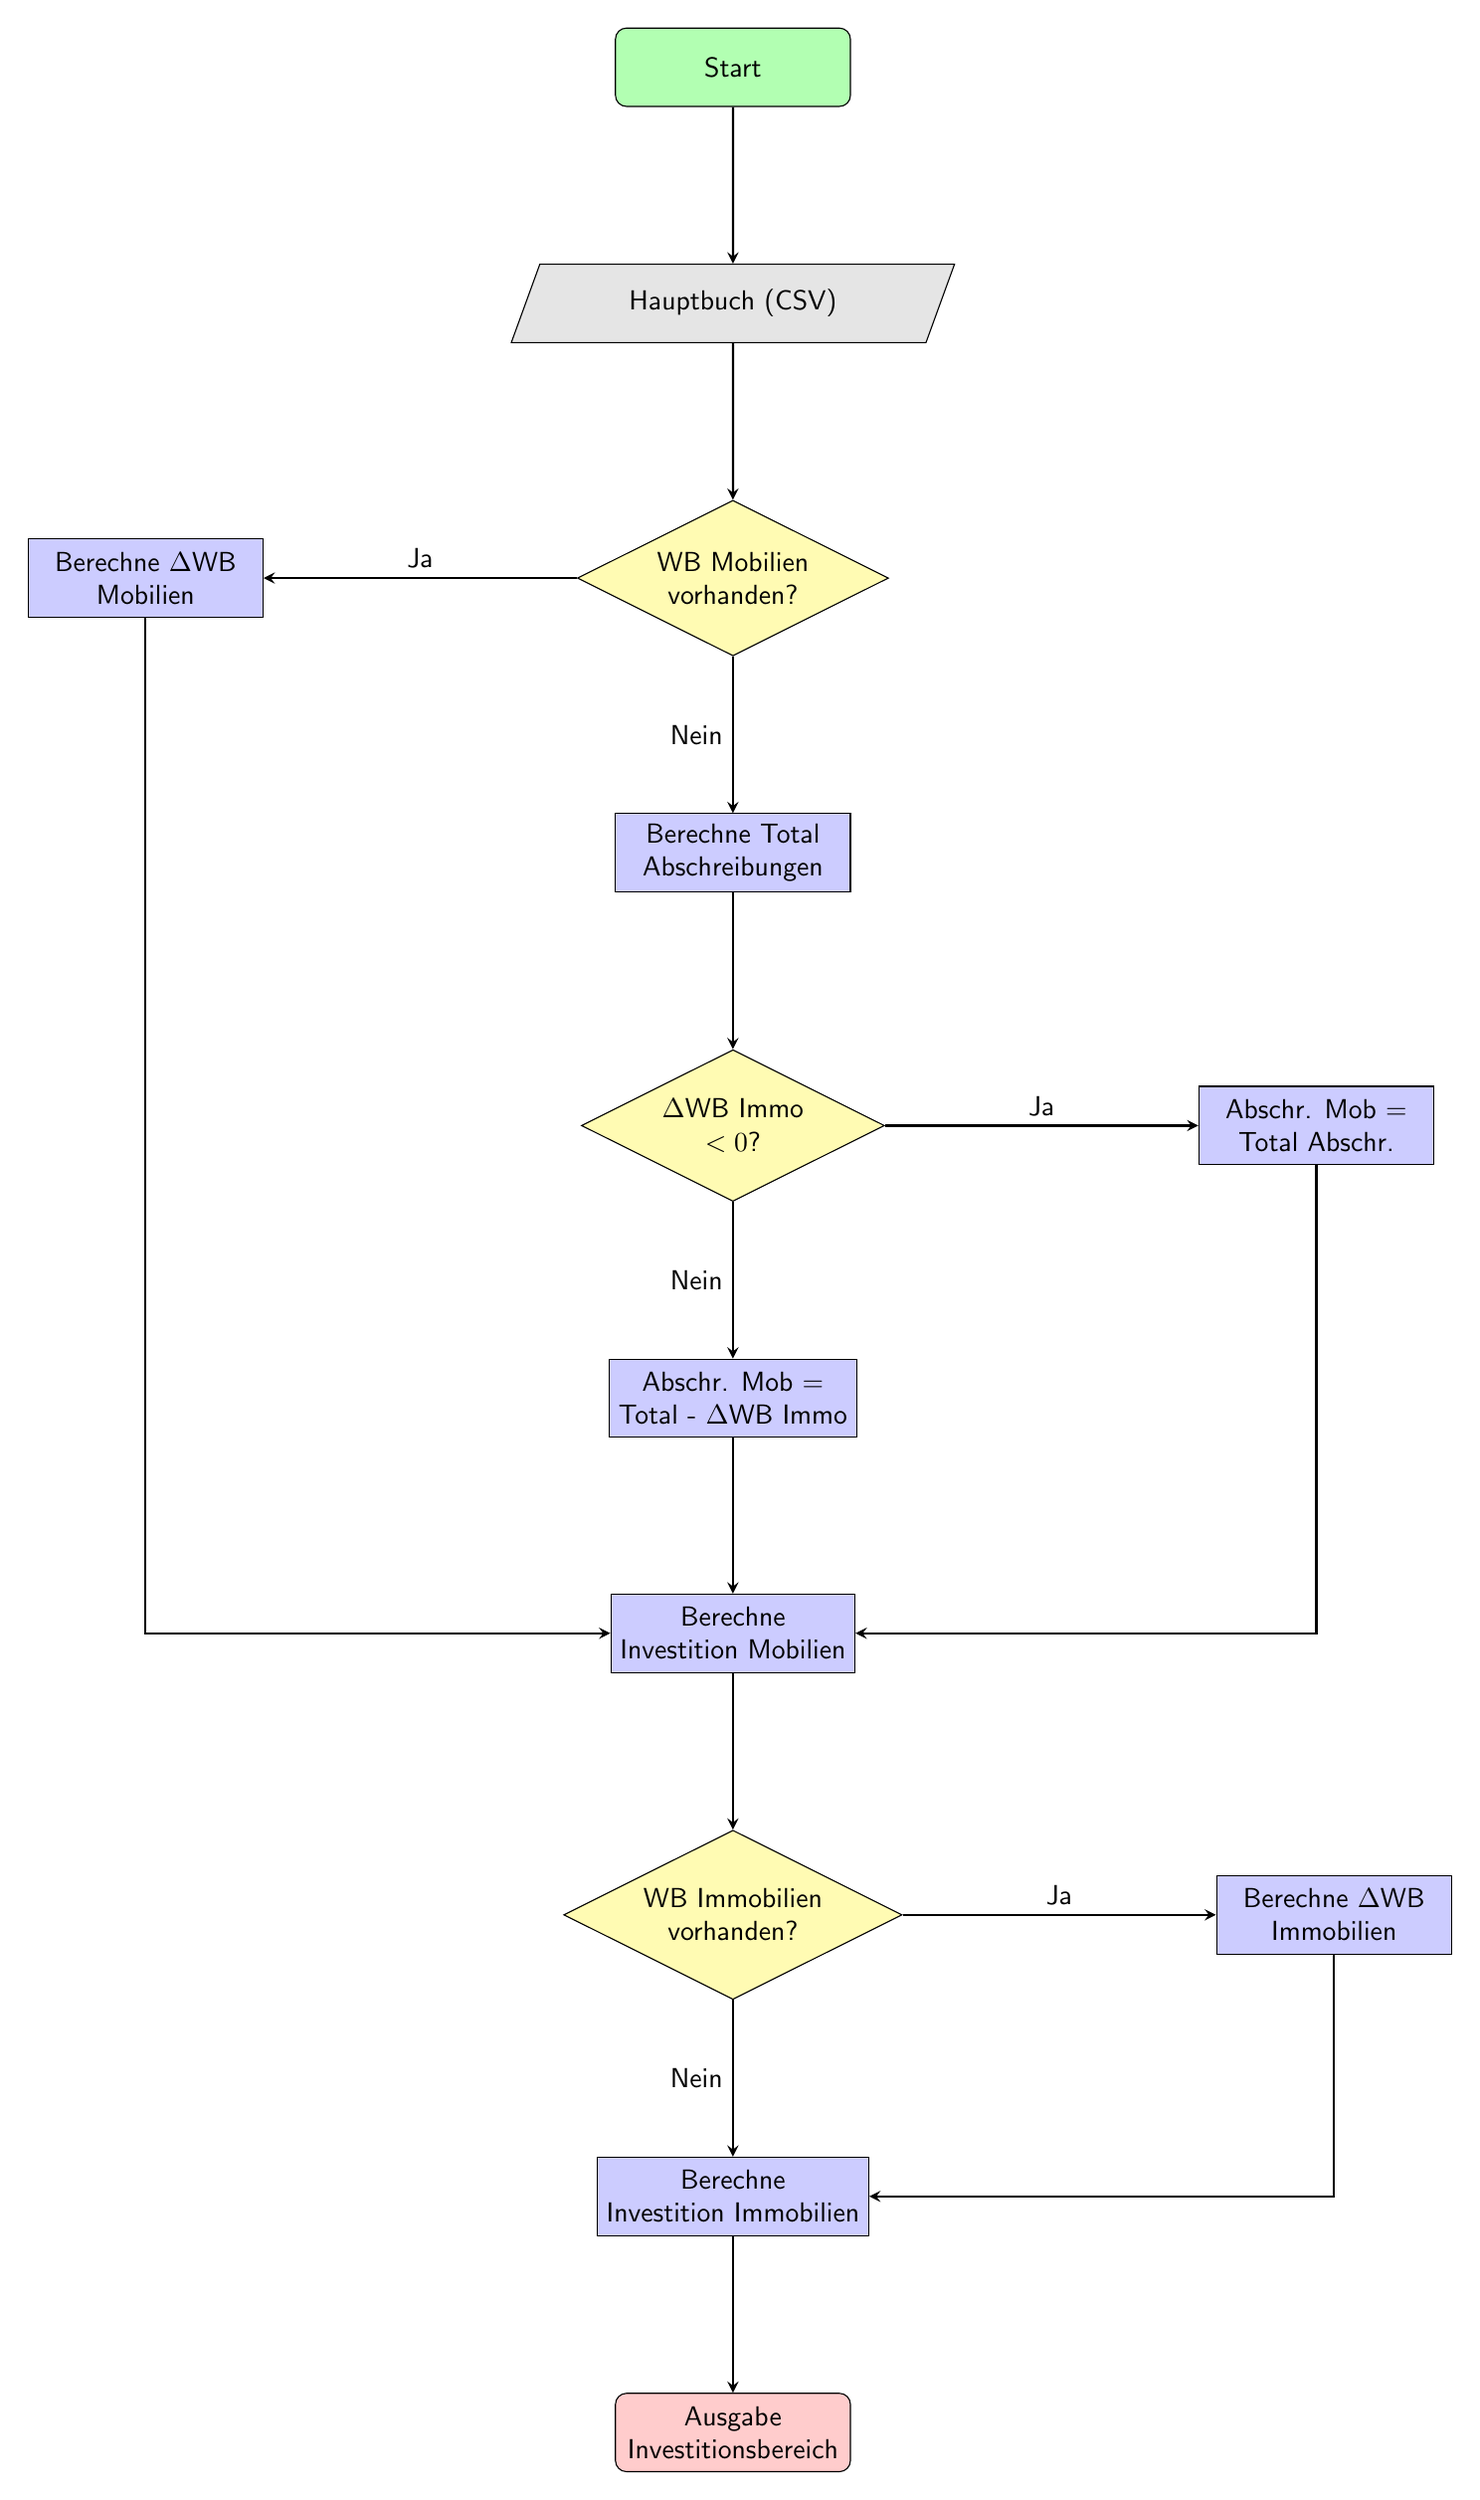
\begin{tikzpicture}[node distance=2cm]

% Start node
\node (start) [start] {Start};

% Input data
\node (data) [data, below=of start] {Hauptbuch (CSV)};

% First branch - Check WB Mobilien
\node (check_wb_mob) [decision, below=of data] {WB Mobilien \\ vorhanden?};

% Mobile assets calculation paths
\node (wb_mob_yes) [process, left=4cm of check_wb_mob] {Berechne $\Delta$WB \\ Mobilien};
\node (get_total_absch) [process, below=of check_wb_mob] {Berechne Total \\ Abschreibungen};
\node (check_wb_immo) [decision, below=of get_total_absch] {$\Delta$WB Immo \\ $< 0$?};
\node (absch_mob_all) [process, right=4cm of check_wb_immo] {Abschr. Mob = \\ Total Abschr.};
\node (absch_mob_diff) [process, below=of check_wb_immo] {Abschr. Mob = \\ Total - $\Delta$WB Immo};

% Investment calculation
\node (invest_mob) [process, below=5cm of check_wb_immo] {Berechne \\ Investition Mobilien};

% Immobilien calculation
\node (check_wb_immo2) [decision, below=of invest_mob] {WB Immobilien \\ vorhanden?};
\node (wb_immo_yes) [process, right=4cm of check_wb_immo2] {Berechne $\Delta$WB \\ Immobilien};
\node (invest_immo_calc) [process, below= of check_wb_immo2] {Berechne \\ Investition Immobilien};

% Output
\node (output) [output, below=of invest_immo_calc] {Ausgabe \\ Investitionsbereich};

% Arrows
\draw [arrow] (start) -- (data);
\draw [arrow] (data) -- (check_wb_mob);
\draw [arrow] (check_wb_mob) -- node[above] {Ja} (wb_mob_yes);
\draw [arrow] (check_wb_mob) -- node[left] {Nein} (get_total_absch);
\draw [arrow] (get_total_absch) -- (check_wb_immo);
\draw [arrow] (check_wb_immo) -- node[above] {Ja} (absch_mob_all);
\draw [arrow] (check_wb_immo) -- node[left] {Nein} (absch_mob_diff);
\draw [arrow] (wb_mob_yes) |- (invest_mob);
\draw [arrow] (absch_mob_all) |- (invest_mob);
\draw [arrow] (absch_mob_diff) -- (invest_mob);
\draw [arrow] (invest_mob) -- (check_wb_immo2);
\draw [arrow] (check_wb_immo2) -- node[above] {Ja} (wb_immo_yes);
\draw [arrow] (check_wb_immo2) -- node[left] {Nein} (invest_immo_calc);
\draw [arrow] (wb_immo_yes) |- (invest_immo_calc);
\draw [arrow] (invest_immo_calc) -- (output);

\end{tikzpicture}
\end{document}
